\documentclass[paper=a4, parskip=half-]{scrartcl}
\usepackage[utf8]{inputenc}

\usepackage{amsmath}
\usepackage{mathtools}
\usepackage{marvosym} % for the \Lightning symbol
\usepackage{amssymb} % more icons/symbols
\usepackage{tablefootnote} % for footnotes in tables
% not in standard texlive, can't be asked to figure it out now
%\usepackage{ccicons} % creative commons icon
\usepackage{hyperref} % for hyper links
\usepackage[dvipsnames]{xcolor} % to color stuff -- dvipnames for additional color names
\usepackage[shortlabels]{enumitem} % to modify enumeration labels
\usepackage{tcolorbox} % for colored boxes - see https://tex.stackexchange.com/questions/66154/how-to-construct-a-coloured-box-with-rounded-corners/172608#172608
\usepackage{tikz} % drawing stuff
\usepackage{eurosym} % € (no, default LaTeX font doesn't include it)
\usepackage{natbib}
\usepackage{graphicx}

\usepackage{listings}

\usepackage{geometry}
 \geometry{
 a4paper,
 left=20mm,
 right=20mm,
 top=20mm,
 bottom=30mm,
 }


\title{Data Management Systems}
\author{\texttt{\{wnicole\}@ethz.ch}}
\date{ETH Zürich, HS 2020}

% Custom commands
\newcommand{\setzeroone}{\lbrace 0, 1 \rbrace} % => {0,1} (Notice the missing $$)
\newcommand{\horizontaldivider}{\begin{center} \line(1,0){350} \end{center}}

\begin{document}

\begin{titlepage}
\maketitle
\vspace{5cm}
\thispagestyle{empty}


\begin{abstract}
This is a summary for the course \textit{Data Management Systems} at ETH Zürich.

I do not guarantee correctness or completeness, nor is this document endorsed by the lecturers. Feel free to point out any erratas. It's probably smart to reread your old DMDB summary first!
\end{abstract}

\end{titlepage}

\tableofcontents
%\listoffigures
%\listoftables
\newpage

\section{Introduction}

\subsection{Introduction}

This course is about all the architectural components of a database management system. While the DMDB Bachelor course was mostly about basic, abstract and high-level concepts, this course goes deeper into the importance of the architectural design of a DBMS. This includes principles on how to (efficiently) store data on disk and memory, how to move data from disk to memory, processing and optimizing queries, understanding the underlying concepts of query operators, concurrency control and recovery. Figure \ref{fig:arch} is an overview of the architectural components of a DBMS and for a more detailed graphic refer to Figure \ref{fig:arch2}. Some basic terms are explained in the following few paragraphs.

\begin{figure}[h]
	\centering
	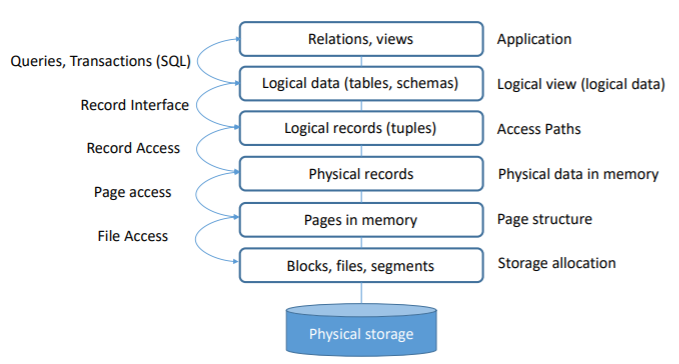
\includegraphics[scale=0.8]{images/00-arch.PNG}
	\caption{Architecture of a DBMS.}
	\label{fig:arch}
\end{figure}

\paragraph{Database Management System (DBMS)}
Tool that helps develop and run data-intensive applications. A DBMS pushes the complexity of dealing with the data (storage, processing, consistency) to the database rather than to the program.

\paragraph{Data Independence}
User applications are immune to changes made in the definition and organization of data. A DBMS provides an abstract view of the data that hides details of data representation and storage.

\paragraph{Logical Data Independence}
The logical structure of data is known as the schema definition (see below). Independence refers to the ability to modify the logical schema without causing application programs to be rewritten. A database allows to build views over the schema s.t. different logical interpretations of the same data are possible. E.g. adding a new column to one user will not change the outcome for another user.

\paragraph{Physical Data Independence}
The ability to modify the physical schema (e.g. to improve performance) without causing the application programs to be rewritten i.e. without affecting the conceptual / external view of the data. The database hides how the data is actually stored persistently and represented in memory.

\paragraph{Schema}
Organization of data, i.e. a blueprint of how the DB is constructed. The formal definition is a set of integrity constraints. In a relational DB, the schema defines elements like tables, fields, relationships views, indexes, etc. The schema is generally stored in a data dictionary. Most common examples include:

\textbf{Flat Model:} Two-dimensional array, elements in each column have the same data type and elements of same row relate to each other. I.e. a single DB table with no relations.

\textbf{Hierarchical Model:} Tree with one-to-many relationships between parent and child nodes. I.e. an XML / JSON file.

\textbf{Network Model:} The above but with many-to-many relationships a.k.a. a graph, potentially with cycles.

\textbf{Relational Model:} We all (should) know what this is.

\textbf{Star Schema:} One or more fact tables (quantitative data) referencing any number of dimension tables (descriptive attributes related to fact data). E.g. a DB of sales: each sale is a fact with date, store, product, etc. and each fact-field is connected to a dimension table that describes that fact field (date dimension would be day, month, year, etc.). A RDBMS can be structured into a star. Mostly used for OLAP. Special Case of a snowflake schema.

\textbf{Snowflake Schema:} Star schema with normalized dimensions, i.e. a single dimension field can be connected to another entire dimension table.

\paragraph{Declarative Language}
SQL is a declarative language and specifies how the result looks like while describing the tuples that should be part of it. A DL does not specify how to get to the result (i.e. no control flow, only logic of a computation - what, not how). With this, the DB can optimize queries.

\paragraph{Function and Data Shipping}
In a distributed system (see parallel architectures below), resources have to be used optimally for efficient query processing. Function shipping refers to processing the data close to where it is actually stored with the results being sent back to the requester. Data shipping refers to moving data to the place where it is processed (as in shared-disk architectures since data needs to be moved from disk to memory to be processed). Both concepts can be combined (as in shared-nothing architectures).


\subsection{Reading Assignments}

For this section, there is only one reading assignment and it is pretty long. It is incredibly helpful though and provides a good overview on almost all the topics discussed in this course. Link \href{https://dsf.berkeley.edu/papers/fntdb07-architecture.pdf}{here}. Most topics are scattered across the next Sections.


\subsubsection{Architecture of a Database System}

\begin{figure}[h]
	\centering
	\includegraphics[scale=0.9]{images/00-arch2.PNG}
	\caption{Main components of an RDBMS.}
	\label{fig:arch2}
\end{figure}

\paragraph{Life of a Query}
We move down and up in the following stack to handle a query:
\begin{enumerate}
    \item Client calls API that communicates over a network to establish a connection with the \textbf{Client Communication Manager}, which responds to SQL commands and returns data / control messages.
    \item The \textbf{Process Manager} assigns a thread of computation to the command if there are enough resources to handle it or delays it until there are.
    \item The \textbf{Relational Query Processor} checks if the user is authorized to run the query, compiles the SQL text to an internal query plan and executes it. Query processing is handled by operators implementing certain tasks (join, selection, tuple fetching, etc.).
    \item The \textbf{Transactional Storage Manager} handles operator requests to write and read data pertaining to the ACID principles (lock manager). It includes algos and data structures defining how to access data on disk (access methods), buffer data (bringing it from disk to memory - how and when) and recover it in case of failure (log manager).
\end{enumerate}

\paragraph{Processes vs. Threads}
\begin{itemize}
    \item \textbf{OS Process:} A program execution unit scheduled and managed by the OS kernel \footnote{Kernel: core program of an OS with complete control over everything in the system. It connects the application software to the hardware (CPU, memory, devices).} with a private and unique address space and its own state. OS processes can share physical memory but not virtual memory. Context switching is complex and expensive.
    \item \textbf{OS Thread:} A program execution unit part of a multi-threaded process that shares its address space and context with other threads from the same process. Scheduled and managed by the kernel. Context switching is easy and fast.
    \item \textbf{Hyperthread:} A concept in multicore systems (multiple CPUs in one processor). Hyperthreading allows for simultaneous multithreading. %TODO better?
    \item \textbf{Lightweight Thread Package:} Threading in a user-space context. One single OS process managed by the kernel contains the user-level threads that are scheduled by a user-level scheduler (also a thread in the OS process). In the DBMS context it means that the DBMS implements its own multithreading.
    \item \textbf{Client Process / DBMS Client:} Execution unit running on client / application side used to connect to the DB engine.
    \item \textbf{Server Process / DBMS Worker:} Execution unit running inside the DB engine, used to execute queries on behalf of a client. A query can be processed by several server processes (parallel execution) a.k.a. a pool. Many-to-many also possible (each worker has own specialized task handling many queries).
    \item Potentially confusing: the two things above can also be threads in a DB context! See below to see the different models.
\end{itemize}

\paragraph{Process Model}
How to map client and workers. The following models work for uniprocessor systems.

\paragraph{OS Process per DBMS Worker}
Workers are mapped directly to OS processes. Isolation and easy debugging provided. Complicated by numerous shared in-memory structures usually part of a DBMS (lock table, buffer pool, ...) - need to be allocated explicitly in shared-memory. Not scaleable since a process has a bunch of state (memory overhead). Complex context switches.

\paragraph{OS Thread per DBMS Worker}
Workers are mapped directly to OS threads by a dispatcher thread - all part of a single OS process. Needs good threading support from OS. Usual complications as seen in multithread programming. No protection, tricky debugging (race conditions), possible porting difficulties. Scales well. Easy data sharing since all threads run in same address space anyway.

\paragraph{Process Pool}
Central process holding all connections and each SQL request is given a separate process from the pool. Process pool size is bounded (often fixed). Advantages of process per worker with less memory overhead (smaller number of processes required) and less overhead when assigning a process to a client request. Less scaleable than process per worker because of fixed pool size. Thread pools are also possible (more scaleable, better memory sharing / management). 

\paragraph{Lightweight Threads}
If OS thread support is bad, do your own multithreading. Each thread needs to be programmed to manage its own state, to perform potentially blocking operations via non-blocking, asynchronous interfaces and to frequently yield control to a scheduling routine that dispatches among these tasks. Fast task switching and ease of porting but you probably need to replicate a good deal of OS logic in the DBMS.

\paragraph{Parallel Architectures (Multiprocessor System)}
\begin{itemize}
    \item \textbf{Shared-Nothing:} Each node has its own CPU, RAM and disk. All nodes are connected via some kind of network. Each node can run its own process model. Data can be partitioned (hash, range, horizontal / vertical, etc.) across nodes (see function / data shipping above). Easy to maintain and to scale, ideal when data can be partitioned / replicated and updates are not frequent.
    \item \textbf{Shared-Memory:} All processors and disks have access same single RAM, connected with a memory bus (or network). All process models work well for it (except lightweight threads since they're constrained to one processor). Hard to scale because of the shared memory bus (bottleneck). Combining multiple shared-memory clusters is referred to as the hierarchical model.
    \item \textbf{Shared-Disk:} Each processor has own private RAM and all processors are connected to single disk. No complex partitioning, failure resistant. Needs cache coherency mechanisms and distributed lock manager facility to handle data sharing. Needs data shipping. Very common for cloud architectures. Separates storage from compute.
    \item \textbf{NUMA:} Middle ground between shared-nothing and shared-memory - nodes have own fast local memory along with delayed access to some shared memory. Easy to program, scale since they avoid shared points of contention (memory bus). %TODO better?
\end{itemize}


\subsection{Exercises}

\subsubsection{Introductory Topics}

All questions and answers are covered by the sections above.

\newpage

\section{Storage Management}

\subsection{Introduction}

A big part of the performance of databases arises from proper storage management (movement through hierarchy), adequate data representations and suitable optimizations on organizing the data in memory and disk.

Databases provide the illusion of large memory capacity and try to hide the performance problems created by implementing desirable properties (high bandwidth for sequential and concurrent access, low latencies for random accesses, persistent, etc.) through complex architectures and optimizations. Two key guarantees we want to have provided by a DB storage system are: persistent and recoverable data (even in the event of a failure). We would also like physical data independence.



\subsection{Memory Hierarchy}

Databases go through the entire memory hierarchy frequently. Enhance locality (data organization, query scheduling), make sure data is available at layer where it is needed (pre-fetching), be clever about what to keep at each layer (caching, replacement) and keep track of modifications and write back to the lower layers (to persistent storage) when needed.

\begin{figure}[h]
	\centering
	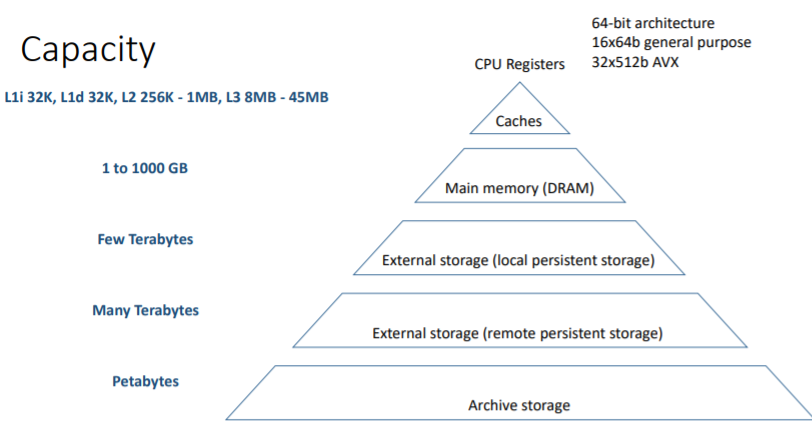
\includegraphics[scale=0.5]{images/1-cap.PNG}
	\caption{Memory hierarchy capacities.}
	\label{fig:cap}
\end{figure}

\begin{figure}[h]
	\centering
	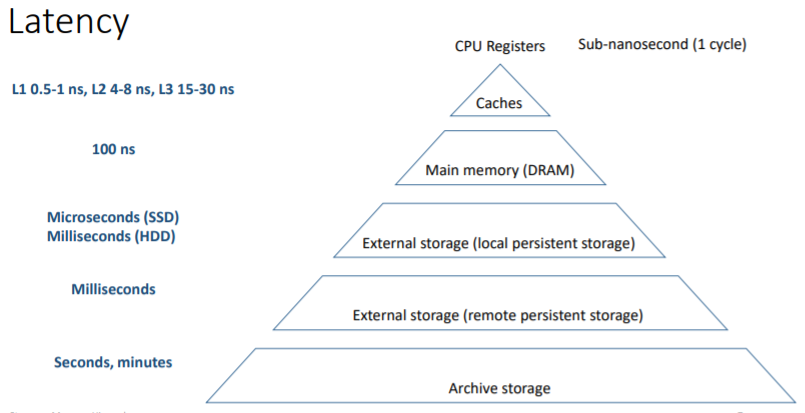
\includegraphics[scale=0.5]{images/1-lat.PNG}
	\caption{Memory hierarchy latencies.}
	\label{fig:lat}
\end{figure}

\begin{figure}[h]
	\centering
	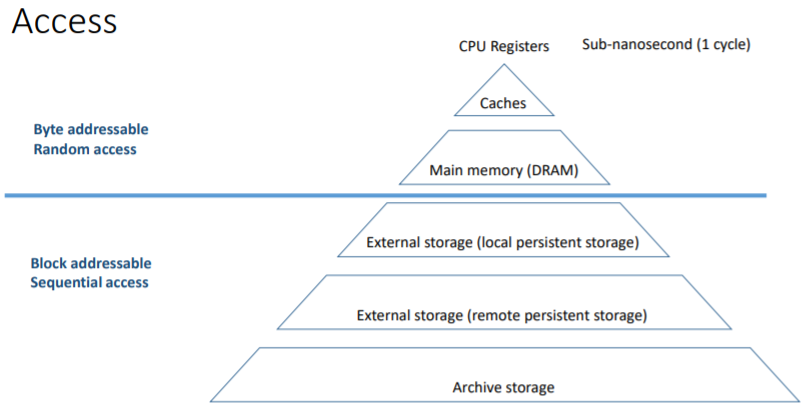
\includegraphics[scale=0.5]{images/1-acc.PNG}
	\caption{Memory hierarchy access methods.}
	\label{fig:acc}
\end{figure}

\paragraph{Memory Wall}
Main memory suffers from several issues: there is never enough of it (application growth), memory outside the CPU chip (DRAM) is much slower than memory located inside of it (latency issue), processor-memory gap (processor speed increases faster than memory speeds - bandwidth is an issue), increased cost (DRAM is expensive) and main memory is not persistent.

\paragraph{Spatial Locality}
Put together what belongs together.

\paragraph{Temporal Locality}
Do at the same time things that require the same data.

\paragraph{Non-Volatile Memory (NVM)}
Located between DRAM and local external storage - combines characteristics of both. Byte addressable, random access, persistent, etc.

\paragraph{Cloud Computing}
Network between compute and storage layer. Ephemeral nature of computing infrastructure forces a separation of compute and storage. Flexibility is provided by cloud provider.

\paragraph{Network Attached Storage (NAS)}
Networks are becoming faster with more bandwidth than storage devices (e.g. RTT in a data center less than a seek operation on a HDD). Eventually, it might be faster to get data from the memory of a remote machine / storage device than from local disk. See also: Remote Direct Memory Access (RMDA).

\paragraph{Multicore and NUMA}
%TODO potentially

\paragraph{Hardware Acceleration}

\paragraph{SSD}






\subsection{Logical Storage Organization}

See the first layer in Figure \ref{fig:arch}. Assumptions: the standard database architecture is based on slow hard drive disks (HDD) that have a high latency for seek operations (random access) - most of the DB is \textbf{not} in memory.

Disclaimer: most explanations from the lecture are based on a real system (Oracle Database)\footnote{For logical storage click \href{https://docs.oracle.com/en/database/oracle/oracle-database/19/cncpt/logical-storage-structures.html#GUID-4AF2D61A-8675-4D48-97A4-B20F401ADA16}{here} and \href{https://docs.oracle.com/cd/B19306_01/server.102/b14220/logical.htm}{here} and for disk storage click \href{https://docs.oracle.com/cd/B19306_01/server.102/b14220/physical.htm}{here} and \href{https://docs.oracle.com/en/database/oracle/oracle-database/19/cncpt/physical-storage-structures.html#GUID-008A1F08-9C75-4E9F-A70B-41FB942C60B4}{here}.}. %TODO look at these pages

Problem statement: a DB is doing many things at the same time and each thing (query, system process, DB component, etc.) active at any point in time needs its own logical view of the data. A DB creates such virtual, logical views of the system using its own mechanisms.

\paragraph{Logical and Physical Storage}
For Oracle 19, those two components are represented by an ER diagram seen in Figure \ref{fig:erdiag} with a crow foot implying a one-to-many relationship). 

A given logical object in a DB (table, index, etc.) is "stored" in a tablespace, a tablespace is organized into segments, segments have space allocated to them in the form of extents and extents are sets of contiguously allocated data blocks.

\begin{figure}[h]
	\centering
	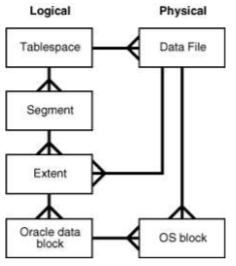
\includegraphics[scale=0.8]{images/1-erdiag.PNG}
	\caption{Oracle 19 logical vs. physical storage.}
	\label{fig:erdiag}
\end{figure}

%TODO more images?


\paragraph{Page}
There are different notions for a page:
\begin{itemize}
    \item \textbf{Hardware Pages:} The atomic unit to write to storage, usually 4KB. Also called block sometimes. Part of a file resp. disk sector.
    \item \textbf{OS Page:} The unit used by the OS to implement virtual memory, usually 4KB.
    \item \textbf{DB Page:} Equivalent to a block, anywhere between 512B and 32KB. Trend is towards larger block sizes since they incur less overhead (less keeping track).
\end{itemize}

\paragraph{Tablespace}
Data unit in a DB which provides a logical representation of the principle of spatial locality (not necessarily stored continuously!) - some form of virtual memory. Data stored is either schema related (table, index, clustered tables) or engine related (data structures for the engine, e.g. result buffers). Space (memory / disk) is allocated to tablespaces. Keep together what needs to be kept together = logical locality = one address.

\paragraph{Segment}
An object in the schema (or part of an object if it is partitioned). Consists of one or more extents (that can be in different data files). Segments allocate (virtual) space to objects. Usually when allocating space, a DBMS gives a little bit more to have some growing space. Even if a table is partitioned into several segments across various disks, the table still has only one tablespace.

\paragraph{Extent}
A collection of physically continuous data blocks (size = tunable /dynamic parameter). Extents are mapped to one data file. Usually when allocating space for an extent, a DBMS gives a little bit more to have some growing space (1.25x common).

Extents are a compromise between static file mapping and dynamic block mapping. I.e. do static mapping to a set of blocks and if more space is needed dynamically do another static mapping connected to the first one. Needs an array of pointers = extent directory (which also needs space - want to keep it small).

\paragraph{Block}
The smallest amount / unit of physical space allocation. Kinda the same thing as a page in an OS - just bigger. The block size is a tunable parameter. With a small block size, you need to keep track of many physical locations and less actual sequential access. With a big block size, you will have fragmentation but more actual sequential access.

\paragraph{Block Structure: Slotted Pages}
A block has a header (address and type of segment, e.g. index, table, etc.), a table directory (schema of the table stored in the block), row directory (pointers to the actual tuples stored in the block (block, slot), data can be anywhere), free space and row data (tuples stored in the block). The directory grows downwards and the space for the tuples grows upwards.

No assumptions can be made on storage order of a table within an extent! E.g. if a tuple is deleted a new one can take its place that has been inserted much later.

\paragraph{Optimizing Block Usage}
\begin{itemize}
    \item \textbf{Percentage Free (PCTFREE):} Allow row inserts until x\% of the space is occupied and leave the rest for updates to existing rows in the blocks. Avoids fragmentation occurring from updates that make an already existing tuple larger. 
    \item \textbf{Percentage Used (PCTUSED):} Determines how much space needs to be free before free space is used to insert new tuples. No more new inserts until used space is under x\%. Avoids having to constantly move a block from the used to the free list and vice versa (costly operation).
    \item These two concepts are often combined. They are a trade-off between efficiency and space.
\end{itemize}

\paragraph{Fragmentation Within Blocks}
Blocks can suffer from fragmentation. Compaction is expensive and only done when the block has enough space for an insert / update but the space is not contiguous. In case of an update not fitting the original block anymore, the tuple is put into a new block with a row pointer in the original space s.t. the ID of the tuple does not need to change (needs indirection) - too much of this slows down access since it multiplies I/O by a factor of at least 2.

\paragraph{Finding Space}
Segments contain one or more free lists that keep track (with pointers) of blocks that have usable free space (not done at an extent-level because the search for space would be more complex). Using several free lists helps avoid contention when performing parallel inserts / updates, e.g. different lists for different actions. Free lists are updates as transactions execute insert / delete / update statements using the rules established with Percentage Free and Percentage Used.

\paragraph{Writing to Disk}
A DB provides concurrency control (DB correct even if several transactions modified data at the same time) and recovery (data can be recovered even after a failure). More details in later sections.

\textbf{Shadow Paging:} When updating an attribute, copy it to a free slot (= page) and update it there. Once the transaction commits, mark the old slot as free and the new one as correct. Only makes sense when the overhead of creating a new copy and managing them is small enough (main memory, flash, NVM, etc.).

\textbf{Delta Files:} A copy of the attribute that is to be updated is stored in a delta file (instead of a free slot in the extent). The update is performed directly on the original value and the copy in the delta file can be discarded if it's no longer needed. Old data in delta file favors commits, simplifies undos and allows looking at older data. New data in delta file favors aborts and allows to delay the propagation of updates.\footnote{Oracle used rollback segments (segments used to store old copies of data) and now switched to undo-tablespaces.}












\subsection{Database Buffer Cache}

See second layer in Figure \ref{fig:arch}. To process data, it has to reside in memory. Since not all the data fits into memory, databases cache blocks in memory and write them back to storage when dirty or in need of more space. So, to provide efficient access to pages, a DBMS implements a large shared buffer pool in its own memory space. A buffer pool is organized as an array of frames, each of the size of a DB disk page. The buffer cache is not used for actual processing - intermediate results are stored in the database heap (region of memory where queries actually work on the data).

Similar to OS virtual memory / paging mechanisms but a DB has much better knowledge about access patterns and the process can be optimized to a larger extend.

It is important to keep the overhead of data structures in mind that are needed to keep track of things.

\paragraph{Buffer Manager}
The buffer manager does all the bookkeeping of the buffer pool and is implemented as a hash table. The table maps page numbers currently held in memory to their location in the frame table, the location for that page on disk and additional metadata associated with the page. The metadata includes a dirty bit indicating the data on the page has been modified and info needed by the chosen replacement policy (pin count, statistics, etc.).

\begin{figure}[h]
	\centering
	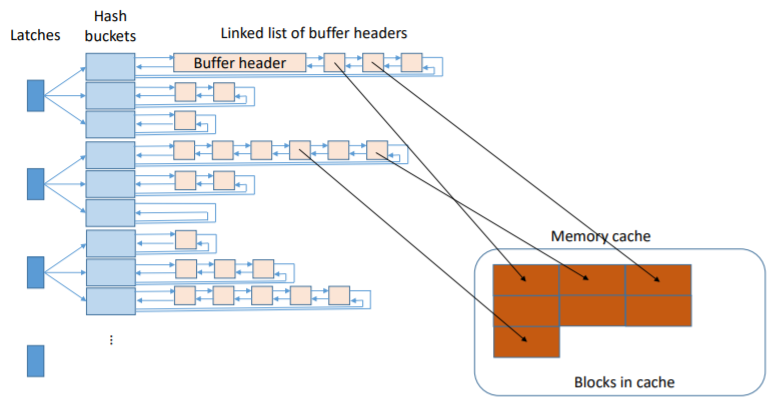
\includegraphics[scale=0.8]{images/1-buffer.PNG}
	\caption{Architecture of a DB buffer manager.}
	\label{fig:buffer}
\end{figure}

\paragraph{Hash Table}
To check if a block is in memory, we take its ID and hash it. Look up the position indicated by the resulting value to check. This is the first check we need to do when processing data.

\paragraph{Latches}
Mechanism to access hash table(s) without the risk of a conflicting concurrent access (similar to a lock)\footnote{Locks usually avoid conflicting updates to data by transactions, while latches avoid conflicting updates in system data structures.}. A latch usually covers several hash buckets (tunable parameter). Latching per bucket or even per block header results in too much overhead since there are so many.

\textbf{Performance Issues:} To check if a block is in memory, a latch needs to be acquired. Since a latch can be only owned by one process, this process blocks several linked lists of block headers. Contention on these latches may cause performance problems (hot blocks, SQL statement accessing many blocks, similar statements executed concurrently, etc.).

\textbf{Mitigation:} Reduce amount of data in the block (with PCTFREE / PCTUSED), more latches and less buckets per latch, multiple buffer pools, tune queries to minimize number of blocks accessed (avoid table scans), avoid many concurrent queries / transactions accessing same data, etc.

\paragraph{Hash Bucket}
Correct linked list storing block header is found by hashing on some form of block identifier. 

\paragraph{Buffer Header Double Linked List}
After hashing, the linked list is traversed looking for an entry (block header) for the corresponding block. Keep the lists short since this is expensive (have more buckets). A block header contains lots of info (block number, type, format, LSN, integrity checksum, latches / status flags, buffer replacement info).

Some engines store other types of blocks in the linked lists, e.g. version blocks (updates result in copies with a timestamp inserted into the list, similar to shadow paging), undo / redo blocks for recovery, dirty blocks, pinned blocks, etc.

\paragraph{Block Status}
The following states are relevant for the management of the buffer: pinned (block cannot be evicted), usage count (statistics on specific block), clean / dirty. This info is used when implementing cache replacement policies. 

\paragraph{Cache Replacement Policy}
What to cache, what to keep, how to evict and when, how to avoid thrashing cache with unnecessary traffic.

\textbf{Least Recently Used (LRU):} Keep track of when a block was used in a list - most recently used. When evicting, pick the least recently used block at the bottom. Does not work very well for DBs (in contrast to OSes) since large table / index range scans can pollute the cache without actually needing to re-access the cached data.

\textbf{Modified LRU:} Put rarely accessed data (statistics) at the bottom of the list or simply don't cache large tables. Or sort blocks according to access frequency instead of simple counters.

\paragraph{Optimizations}
\begin{itemize}
    \item Keep Buffer Pool: tell DB which blocks are important and should not be evicted (separate buffer).
    \item Recycle Buffer Pool: tell DB which blocks should not be kept after they are used (separate buffer).
    \item Keeping statistics of usage of tables and let system decide automatically what should / shouldn't be cached.
    \item Choose clean pages when needing to evict since it's faster (no write to storage).
    \item Ring Buffers: for scans, allocate the pages in a ring s.t. blocks are allocated only within the ring. Full buffer - evict pages from beginning of the ring as they have already been scanned.
    \item Since block sizes are not homogeneous, require a buffer cache for each block size for more space efficient replacement and simple management.
\end{itemize}

%TODO p. 24, read ahead and stuff, interactions

\paragraph{Touch Count (Hot / Cold List)}
A more sophisticated LRU. Insert new blocks in the middle of the list and keep a count of accesses. Frequently accessed blocks float to the top while rarely accessed ones sink. To avoid counting problems (many accesses only for a short amount of time), only increment counter after a (tunable) number of seconds. Periodically decrease counters.

\paragraph{Second Chance}
Strategies similar to LRU can become a bottleneck if the lists are large. With second chance, no list is maintained and counters are kept in the blocks. Buffer is treated as a circular buffer with an eviction process going around. When a page is accessed, counter = 1. When eviction process passes, if counter is 1, set to 0 - if 0, evict page.

\paragraph{Clock Sweep}
Same as second chance but takes into account that some pages are accessed frequently at regular intervals - uses a counter (with tunable max) instead of a 1/0 flag. Increase counter when touched, decrease when eviction passes, evict when counter = 0.

\paragraph{2Q: Using Two Lists}
Use a FIFO list for blocks that do not need to be kept and a LRU list for blocks that are accessed several times. If a block in the FIFO list is accessed again, it is moved to the LRU list. Blocks at the bottom of the LRU list are either moved to FIFO list (or immediately evicted). Evictions happen on FIFO list level.



\subsection{Storage Techniques in Context}

Instead of using physical storage, we are now looking at using a cloud storage and file system (such as Amazon S3). The previous material is put into context with a modern example of a database, namely \textit{Snowflake}.

\paragraph{Snowflake}
A data warehouse specialized for analytical queries developed entirely on the cloud (cloud native). Separates compute (nodes running VMs with a local disk) from storage (Amazon S3).

The query processing layer (compute) is made up of virtual warehouses, with each consisting of a collection of worker nodes (EC2 instances in Amazon). Each worker node has a cache in its local disk with a simple LRU replacement policy. Metadata in the cloud services level tells us where things are stored. %TODO right?

\begin{figure}[h]
	\centering
	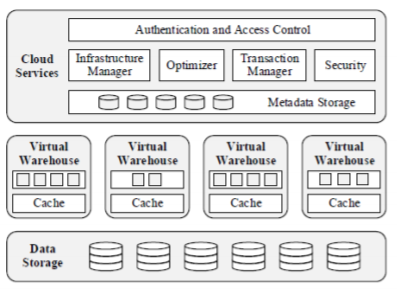
\includegraphics[scale=0.8]{images/1-snowflake.PNG}
	\caption{Snowflake architecture.}
	\label{fig:snowflake}
\end{figure}

\paragraph{Amazon S3 (Simple Storage Service)}
Object storage service in the cloud that acts as he persistent storage that is available to applications. Unlike conventional local disks / distributed file systems (key-value where every object has a key, HTTP(S) PUT / GET / DELETE interface, no updates in place - only full writes that replace old object, can read parts of an object, high CPU overhead because of HTTP, extra expensive I/O because it's network based).
%TODO more?

\paragraph{Micro-Partitions}
Snowflake's extents. To facilitate query processing, they are organized in a special way:

\begin{itemize}
    \item Size ranges between 50 and 500 MB (before compression - data always compressed in S3). In contrast in other DBs, extents are typically in the order of KB.
    \item Each micro-partition has metadata describing what's inside.
    \item Metadata can be read without reading the whole micro-partition.
    \item Metadata is used to read just the part of the micro-partition that is relevant.
    \item Data in micro-partition is stored in columnar form (not by rows). This is the preferred storage format for analytics, improves cache locality, enables vectorized processing, facilitates projection operations and allows to process only the part of the table that is relevant.
    \item Horizontal partitioning (table partitioned into several MP horizontally) - allows to read the table in parallel and facilitates reading only wanted info.
    \item All of this allows for storage level processing to read only parts of the file that are needed which minimizes data movement to and from storage.
\end{itemize}

\begin{figure}[h]
	\centering
	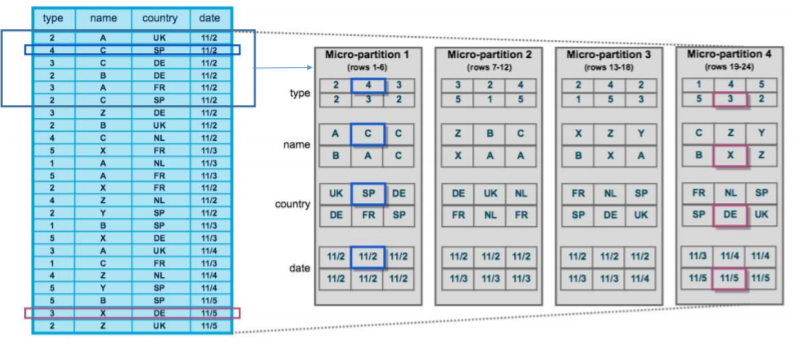
\includegraphics[scale=0.8]{images/1-micropart.PNG}
	\caption{Logical and physical table structure in Snowflake.}
	\label{fig:micropart}
\end{figure}


\paragraph{Pruning based on Metadata}
Example of metadata: in this MP the min. age is x and the max age is y. With a query only wanting all entries with age $>$ y, we can discard that MP. Other examples are: number of distinct values, number of nulls, bloom filters, etc.

Snowflake does not use indexes (requires a lot of space, induce random accesses which are bad for slow storage like S3, need to be maintained and selected correctly). Metadata is much smaller and easier to load.

\paragraph{Writing to Disk}
S3 does not support in-place updates (immutable), an object is replaced in its entirety. Snowflake uses this to implement snapshots of the data (shadow paging): write a new object when MP is modified and keep / discard old MP. Allows for reading of old data and provides fault-tolerance.



\subsection{Reading Assignments}

\subsubsection{An Evaluation of Buffer Management Strategies for Relational Database Systems}

Again: data has to be in RAM for a DBMS to operate on it! A buffer manager intelligently shuffles data from disk to memory. A buffer pool contains frames that can hold pages brought in from disk and are otherwise free. The pool is filled according to some kind of algorithm and replacement policy. A pinned page is a page currently in use - it should not be replaced. Pages that contain modified data are dirty and need to be written back to disk before discarding them.

\paragraph{Domain Separation Algorithm}
Why? Not all pages are the same! Pages are statically classified into types. If a page of type X is needed, allocate it in pool X = domain X. A pool contains several buffers = slots to put the requested pages into. In each domain, LRU is used as the replacement policy. If no slots are available in current domain, borrow slots from another domain.

A suggested type assignment scheme is: assign one domain to each non-leaf level of a B-Tree structure while all the leaves and their data also get one domain.

Cons: Domains are a static concept - the importance of a page may vary across queries - relative importance matters. Partitioning buffers according to domains rather than queries does not prevent interference among competing users. Thrashing is still an issue, there is no load control. There are no priorities among domains (e.g. index page $>$ data page).

\paragraph{Group LRU Algorithm}
The above but with a fixed priority ranking among different groups = domains. Searching for free space always starts at domain with lowest prio.

\paragraph{DS with Working-Sets}
The above but each domain can dynamically vary in size - working-set-like partitioning scheme. Pages in domain i which have been referenced in the last t\_i references are exempt from replacement consideration.

\paragraph{Page-Type Algorithms}
All of the above - TL;DR: they're shit and not really superior to simple LRU or CLOCK.

\paragraph{"New" Algorithm}
Shittiest name ever by the way. Two key observations: The priority of a page is not a property of the page; in contrast, it is a property of the relation to
which that page belongs. Each relation should have a Working Set. 

Buffer pool is subdivided and allocated per-relation. Each relation with buffered pages has a resident set = all buffered pages - replacement policy within each is MRU. Each active relation is entitled to one pinned buffer. Resident sets are linked in a priority list with a global free list on top. High priority (based on some heuristic) is at bottom and less likely to be replaced than top since search for free space starts at top.

Cons: MRU. How to assign prios? List search. No regard for multi-user use case. TL;DR: it has a shitty name AND it is shitty. It's 2 AM and I'm tired.

\paragraph{Hot Set Algorithm}
Hot set: set of pages over which there is a looping behavior - keep those in memory by allocating a large enough buffer pool. Hot point: plot buffer size vs. number of page faults and observe that at some point the buffer is too small and MRU/LRU is shit which equates to lots of page faults. E.g. nested loop join with seq. scan: hot point = number of pages in inner relation plus one.

Hot points for different kinds of queries can be determined but it depends on replacement algo (MRU works better than LRU sometimes, especially in cyclic loops).

Query receives hot points amount of buffers. New query can only enter the system if there's enough space for it according to its hot set size. Leads to memory under-utilization due to overallocation.

\paragraph{Query Locality Set Model (QLSM)}
A RDBMS supports a limited set of operations and the pattern of page references they exhibit are regular and predictable. Each pattern can be decomposed into a number of simple reference patterns. With this, the size of a locality set can be determined in advance per query (= set of buffered pages associated with a file instance = multiple pages belonging to same table). %TODO examples below, check notes for reference patterns

\textbf{Sequential References:} Pages are referenced and processed one after another. \textbf{Straight sequential (SS):} sequential scan without repetition, set = 1. \textbf{Clustered sequential (CS):} clusters made up of records with same key are scanned multiple times, buffer should keep clusters until scan moves on to next cluster, set = number of records in largest cluster divided by numbers of records per page (blocking factor), FIFO and LRU work best. \textbf{Looping sequential (LS):} repeated sequential scan, buffer needs to keep entire file and if it's too large use MRU, set = total number of pages in the file.

\textbf{Random References:} \textbf{Independent random (IR):} data pages are accessed in a random manner. \textbf{Clustered random (CR):} random accesses of clusters, set = number of records in largest cluster. %IR TODO

\textbf{Hierarchical References:} Sequence of page accesses forming a traversal path from root to leaves of an index. \textbf{Straight hierarchical (SH):} index is traversed only once, one buffer frame is enough, set = 1. \textbf{Hierarchical SS (H/SS):} tree traversal with sequential scan of the leaves, set = 1. \textbf{Hierarchical CS (H/CS):} tree traversal with clustered sequential scan of the leaves, set = same as in CS, but replace record with key-pointer pair. \textbf{Looping hierarchical (LH):} repeated access to index structure, pages closer to root are accesses more frequently. %TODO LH

\paragraph{DBMIN}
See extra notes.







\subsubsection{Native Storage Extension for SAP HANA}

\paragraph{SAP HANA}
Column-oriented in-memory DBMS combining OLTP and OLAP with the possibility to also use row-store. It uses multiversion concurrency control (MVCC) to manage concurrency.

\paragraph{SAP HANA with NSE}
Basically the memory-disk model that we have seen until now. Cold data on disk, hot data in memory, warm data in buffer pool.






\subsubsection{The Snowflake Elastic Data Warehouse}










\subsection{Exercises}

\subsubsection{DBMIN}
% IMPORTANT

\newpage

\section{Access Methods}


\subsection{Introduction}

We are now looking at layer 3 and 4 in Figure \ref{fig:arch}. We know now how data is brought from storage to memory - in this section we focus on how it is represented and organized in memory (how tuples are arranged within blocks and indexes), which impacts processing speed and hardware features that can be used.

\paragraph{Workload}
A DB system and its access methods can be constructed to handle a certain kind of workload (on-line transaction / analytic processing = OLT/AP). The type of workload also influences the choice of hardware. We have:
\begin{itemize}
    \item \textbf{Transactional (OLTP):} Workload is dominated by (large amount of) short transactions with updates and modifications (high I/O), usually point queries (targeting one tuple), sensitive to contention, needs lots of processing power. Fits the traditional design of a relational engine.
    \item \textbf{Analytical (OLAP):} Workload is dominated by complex queries combining many tables, usually only read queries, needs large amount of memory and processing power. Usually uses a data warehouse system.
\end{itemize}

\paragraph{Trade-Offs}
Trade-offs made in a DB design can include:
\begin{itemize}
    \item More compact representations vs. more complex processing.
    \item More indexes vs. more space and less maintenance cost.
    \item Row store for OLTP vs. column store for OLAP.
    \item The amount of unused space to keep for updates / movements.
    \item etc.
\end{itemize}


\subsection{Physical Storage Organization}


\paragraph{Finding a Block}
Each segment has a segment header which contains a (linked) list of used and free blocks. Both lists keep track of block IDs (Extent, Offset) while the free list also keeps track of the available space. This system is a potential bottleneck, especially for modification transactions.

\textbf{Improving Performance:} Using several free lists for faster concurrent transactions, making the traversal of the free list fast (sorting by size, keep it short, etc.), efficient search for holes in all blocks, etc.

\paragraph{Finding a Tuple / Record}
Each block, next to a block header, maintains a list of pointers (offsets) to all the slots in it that store a tuple each. Each tuple has an ID (Block ID, Offset). The slots / tuples are not uniform in size (hence the offsets).

\textbf{Changes:} Too large for the slot - keep a new pointer in original position to new location of tuple (can be in a different block, ID stays the same). Deletion - remove pointer. Smaller - just leave space empty. Insertion - use a block with enough free space (compact it if needed).

\paragraph{Tuple / Record Structure}
A tuple contains a header (validity flags for deletion, visibility info for concurrency control, bit map of null values, etc.) and attributes (data / pointer to data for each non-null attribute) as seen in Figure \ref{fig:tuple}. A relational DB does \textbf{not} store schema information (table name, data types of attributes, number of attributes, etc.) in a tuple - this is in contrast to schema-less systems (see later).

\begin{figure}[h]
	\centering
	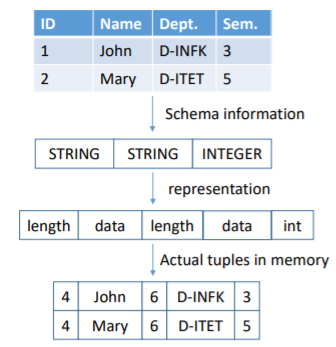
\includegraphics[scale=0.6]{images/2-tuple.PNG}
	\caption{Tuple representation in memory (header omitted - usually in front of data).}
	\label{fig:tuple}
\end{figure}

\paragraph{Record Layout Optimizations}
The serial representation as seen in Figure \ref{fig:tuple} is intuitive but has a linear time to access each attribute. To improve the access time, we can either have a fixed sized part at the beginning of a tuple that stores offsets instead of lengths with each pointer pointing to the tail of an attribute (constant access time for each attribute or simply reorder the attributes such that variable length data (e.g. strings) is placed at the end (again with the pointer system from above). %TODO: how is this constant access if we first have to find out which offset we need?

\paragraph{Data Types}
\begin{itemize}
    \item \textbf{Integer Numbers:} %TODO how representation, similar to C
    \item \textbf{Real Numbers:} IEEE-754 standard for variable precision or fixed point representations for fixed precision (avoids rounding errors). %TODO
    \item \textbf{Strings and BLOBS (Binary Large Objects):} Length and data.
    \item \textbf{Time, Coordinates, Points, etc.:} System specific.
\end{itemize}

When a tuple / single attribute is very big (usually in reference to block size), instead of storing the whole thing one can store the fixed part of it and a pointer to the variable part (potentially in a different block or even a DB-external file). Since it is common that those attributes are not processed by queries, putting them somewhere else speeds up scanning operations. This is usually the case for BLOBS (e.g. pictures, text, etc.).

\paragraph{Row Store}
Tuples are stored as described so far with all the attributes staying together (just as seen as in a table). Allows for quick access and retrieval of an entire tuple. Is usually used in OLTP systems where operations are mostly carried out on individual tuples. When only retrieving a single attribute, a lot of unnecessary data is scanned and brought into the cache since we carry entire blocks.

\paragraph{Column Store}
The data is stored by columns, i.e. each block contains columns instead of rows of a table. Usually used on OLAP / in-memory DBs. Each column either has virtual IDs (order = ID, as in row store, safes space) or explicit IDs which are repeated for each column s.t. each column can be treated individually and (relative) order does not matter. Uses the cache very efficiently. Easy to compress. Improves bandwidth. Disadvantages: When an entire tuple is needed, we need to access several blocks. Complex if a tuple needs to be reconstructed as an intermediate / final result. Modifications are more difficult.

\textbf{Vectorized Processing / SIMD:} Simultaneously performing an operation on a vector of values. Column store is the perfect data representation for this. Very useful for numeric values and bit comparisons.

\paragraph{Partition Attributes Across (PAX)}
An alternative tuple representation as seen in Figure \ref{fig:pax}. A block is divided into mini-blocks and contains several tuples but is organized as a column store. Reconstructing the tuple does not require access to several blocks. See papers (below) for more info.

\begin{figure}[h]
	\centering
	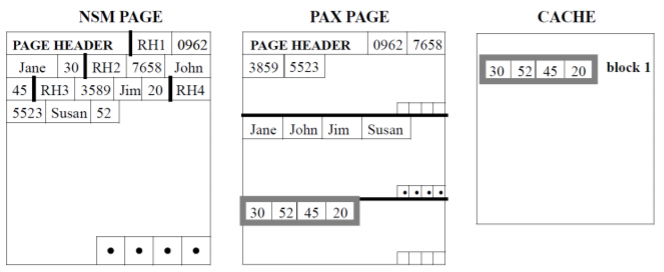
\includegraphics[scale=0.8]{images/2-pax.PNG}
	\caption{Row store (NSM) vs. PAX representation.}
	\label{fig:pax}
\end{figure}

\paragraph{Compression}
Not used to save space but rather to save bandwidth. There is a trade-off between the CPU cycles needed to (de)compress and the memory bandwidth (today: former wins, CPU much faster than memory). There is a possibility to process data in its compressed form. There are many different compression mechanisms and they depend on the data organization (dictionary, run length encoding, delta encoding, bitmaps, etc.).

\paragraph{Dictionary Compression}
Rather an encoding than actual compression. Build a dictionary that maps long entries to, for example, integers / small numbers when the data is loaded. This can be applied to any finite collection of names (e.g. countries, departments, etc.). The data can be easily processed in its encoded form. A hash function is one way to implement a dictionary encoding.

\paragraph{Frame of Reference}
Many attributes have value locality and can be represented as a delta over some base (e.g. 1007, 1017, 1090 represented as 1000, 7, 17 and 90). This allows for operations on compressed data. Can be combined with delta encoding for sorted lists of data (store difference to previous value rather than actual value).

\paragraph{Run Length Encoding}
If a value repeats, store it once and how many time it appears. Useful for attributes with low cardinality (e.g. departments). Often used in column store. For row store it is used for long strings with repeated characters. Compresses the data significantly but processing is more complex. The encoding is variable in size.

\paragraph{Bit-Vector Representation / Bitmap}
For every value that an attribute may take, construct the bitmap as follows: create array as long as number of tuples, if tuple i has value x for that attribute, position i in the bitmap x is set to 1. Bitmaps act as an index and can be used to process queries just by looking at it (selections, joins on an attribute, group by on attribute, etc.). Can be further compressed using run length encoding - but processing becomes more complex.





\subsection{Indexing}

An index is a data structure that improves the speed (sub-linear time) of data retrieval operations (random and sequential) on a database table at the cost of additional writes and storage space (as in B+ Trees) - or processing power (as in hashing) - to maintain the index data structure. It can be stored on either disk or RAM. An index can also be used to police database constraints when data is inserted / updated (i.e. unique, exclusion, primary / foreign key). A DB index is the same concept as an index at the end of a textbook indicating on which page(s) certain topics can be found.

Usually, when data is loaded into storage, it has no order = heap. The records are simply put into empty blocks and when a block is full, move to the next free block. The records of a table can therefore span over multiple physical data blocks residing on disk. Records are accessed by specifying the disk sector, disk row = block (usually 521 bytes) and block offset. An index is another way to logically represent data which has the advantage to make its retrieval more efficient.


\subsubsection{Hashing}

Hashing can be used to construct an index but also as a partitioning strategy when allocating data. A hash is not really an index but it is one way to implement an indexing functionality. A hash index is used to create physical addresses for records (usually using their primary key as input to the hash function).

\paragraph{Hash Function}
A function applied to some kind of arbitrary sized value (e.g. a single attribute value of a table) resulting in a fixed-size hash value. A hash value is usually much smaller than the original value. Different values might result in the same hash value since they are fixed in size (= collision).

There are many functions with strong properties but in a DB the function has to be computationally cheap (usually a modulo operation) since it is used very often.

\paragraph{Hash Table}
A structure that maps keys (usually primary key) to values. It uses a hash function to compute an index for an array of buckets / slots (in DB: bucket = typically a block) that contain the desired values. To look up a desired value, the key is hashed and the location of it is found with the resulting index. This only works for point queries.

Collisions do not happen with perfect hash functions but the table needs to be as big as the cardinality of the attributes (e.g. 4 byte keys = 4 GB table). But if the table is too small, we have too many collisions. Growing the hash table is an expensive operation. Choosing the perfect size is key.

\paragraph{Dealing with Collisions / Static Hashing}
Since a bucket in a DB is usually a block and not a single tuple, i.e. colliding values might simply belong to the same block, we have less "bad" collisions - this usually means that we ran into a block that is full and we to allocate a new one. Ways to deal with such collisions include:

\begin{itemize}
    \item \textbf{Closed Hashing / Chaining:} Add a block with free space to the linked list pointed to by a hash bucket. Not optimal because locating the desired tuple is now more complex (especially if the linked list is long). Improve efficiency by already adding free blocks to a linked list before collision even occurs.
    \item \textbf{Open Hashing:} Look for an empty slot in the hash table using some rule. Linear probing: simply add tuple to the block with index = index + 1. Cuckoo hashing: use several hash functions, if the first one leads to a collision use the next one and so on.
\end{itemize}

\paragraph{Growing the Hash Table / Dynamic Hashing}
This needs to be done when the hash table is completely full. A basic approach would be to create a new, larger hash table with more buckets (typically 2x) and rehash all the existing tuples. Very expensive and inefficient, lots of random accesses and cannot be done on disk (where hash indices are mostly used). Other approaches are often used in combination or in a nested manner (bucket directory pointing to another hash table pointing to actual data - helps with skew).

\textbf{Extendible Hashing:} Instead of having each hash value uniquely identify its own bucket, several hash values point to the same bucket and therefore the same block. If a block fills up, split it and move entries as needed. This increases the available space without significantly changing the hashing mechanism but it requires two page lookups (bucket directory and data block). To allow for more splitting (higher degree of sharing), the size of the table / bucket directory can be doubled by adding another bit to the matching value which increases the number of buckets = logical doubling. %TODO better?

\textbf{Linear Hashing:} A split pointer is used to indicate which bucket will be split in case of overflow (which is not necessarily the one that actually overflows - this one is simply chained) or other triggers (load factor, max. chain length, etc.). The entries targeted by the split bucket use a second hash function targeting the expanded range (mod n, mod 2n). After splitting, move the pointer to the next block. With this, the size of the hash table is gradually increased while redistributing the table (pointer hitting a chained block). The directory grows page by page instead of doubling. Once all buckets have been split, start anew. %TODO better


\subsubsection{B+ Tree Index}

B+ Trees are used to create an index by trading in space. No matter what is said, a DB always uses B+ Trees, never B-Trees. With a B+ Tree index, we always have to specify what we are indexing on (one or multiple attributes). An index sorts the specified attribute value(s) with each row including a pointer to the actual memory location of the block containing the respective record. Pointers can also point to another index and so on. A table can have multiple indexes logically sorting it in many different ways.

It is infeasible to directly sort the physical data (base table) since it can be highly dynamic and we might want to sort it on different (combinations of) attributes for different queries.

One of the best videos to watch is \href{https://www.youtube.com/watch?v=aZjYr87r1b8}{this one}. Explains why and what B-Trees are and how they relate to a DBMS.


\paragraph{Clustered Index / Primary Index}
A clustered index of a table defined on a certain (set of) attribute(s) (predicate) \textbf{physically} sorts the data according to the index when storing it on disk. The leaf nodes (see later) include the actual base table data (divided into blocks, not single rows!). There can only be one clustered index per table. When the clustered index is defined over a set of attributes, it is impossible to access it using a subset of these attributes.

A clustered index is typically created automatically when loading data into the DB using the primary key as the index attribute. Very efficient for data that is not updated frequently. When inserting new values, remaining free space on the blocks is filled and if a block is full, indirection is necessary (see previous sections).

\paragraph{Non-Clustered Index / Secondary Index}
An index defined over a certain (set of) attribute(s) (predicate) with leaf nodes containing pointers to the physical data stored on disk. The physical data may be stored as a simple heap or if a clustered index is present, a non-clustered index may point to the key values present in the clustered index (kinda like two seek operations). There can be multiple non-clustered on different predicates defined on the base table.

\paragraph{Index Key}
An index has to be defined over a certain predicate. It can either be a single attribute (e.g. primary key) or a combination of attributes. A composite key is compared lexicographically:

$$
(a1,b1) < (a2,b2) \Longleftrightarrow (a1 < b1) \lor (a1 = b2 \land a2 < b2)
$$



\paragraph{B-Tree}
Self-balancing tree that maintains sorted data and allows for searches, sequential access, insertions and deletions in logarithmic time. It requires linear space. It is a generalization of a binary tree since it allows for more than two children per node.

\begin{itemize}
    \item Order = $m$.
    \item Every node has at most $m$ children.
    \item Every non-leaf node except root has at least $\frac{m}{2}$ (round up) children.
    \item If it is not a leaf, the root has at least two children.
    \item A non-leaf node with $k$ children contains $k-1$ keys.
    \item All leaves appear in the same level.
\end{itemize}

If a B-Tree is used as an index, each node contains several pointers to data referenced by the keys present in the node (on top of the pointers to the child nodes).

%TODO good example

A B-Tree is constructed bottom up. Whenever a node is full, it is split and the parent node is updated to correctly reference its children.

\paragraph{B+ Tree}
Is a B-Tree where the data is at the leaves only (actual data or pointers to the data). The leaf nodes are organized as a linked list. Each key in the inner nodes is repeated accordingly in the leaves. The values in the same leaf node might point to different data blocks.

Indexes are referred by segments and they can use different block sizes (= nodes) than actual data blocks. Furthermore, an index can have its own memory buffer to avoid that something working on the index affects something working on the data.

%TODO good example


\paragraph{Non-Unique Values}
A B+ Tree index can be built on any attribute including those that are not unique. To differentiate duplicates, we can either repeat the key at the leaf nodes for every duplicate entry or store the key once and let it point to a linked list of all the matching entries. If the data is stored directly in the leaves, append the tuple ID to differentiate tuples the entries are referring to. %TODO what does this look like exactly, reading

\paragraph{Direct Lookup}
To find a single tuple, traverse the tree starting from the root. Within each node, use binary search to look for the correct entry. At the leaf node: return the corresponding pointer / position.

\paragraph{Range Lookup}
To find tuples that are in a particular range, start by finding the leaf node corresponding to the first value and then follow the linked list until we hit the second value.

\paragraph{Insertion}
Lookup the corresponding leaf. If there is space, insert. If there is no space, split leaf into two, insert item and insert new separator on parent node. If parent node is full, split it in two and insert separator in parent's parent node. Go all the way to the root if necessary. %TODO example

\paragraph{Deletion}
Lookup the corresponding leaf and remove entry. If the leaf is less than half order full, check a neighboring leaf. If it is more than half full, balance both. If it is half full, merge both. Update separator(s) in parent. %TODO example

\paragraph{Concurrent Access}
Use lock coupling to protect index from conflicting concurrent accesses. When accessing the index, first lock the root and the first level. Check where you have to go and only then release first lock on root. Lock second level and repeat up to the leaf level. %TODO lock on entire level or on one node of level? %TODO more, splitting p.29/30

%TODO index locking

\paragraph{Creating a B+ Tree Index}
A B+ Tree is created bottom up (leaves first):

\begin{itemize}
    \item Sort the data
    \item Fill blocks one after another (leave space if updates are anticipated else we have a clustered and compact tree)
    \item Remember largest value in each block %TODO or left/right bias
    \item Create inner nodes by using largest value in each block as separator
    \item Iterate upwards to the next level until there is only a single block (root)
\end{itemize}

\paragraph{Optimizations}
\begin{itemize}
    \item \textbf{Reverse Index:} If the indexed attribute is a sequence and new items are constantly produced, insert items by reversing them so that they are more likely to go to different blocks. This protects from concurrent updates fighting to insert on the same block.
    \item \textbf{More Efficient Keys:} Replace keys in inner nodes with shorter separators that have the same effect or factor the children's common prefix. %TODO insert images
    \item \textbf{Ignore Rules:} Don't merge nodes when they do not have enough data - delaying a merge can minimize changes. Periodically rebuild the tree instead. Also: using variable length keys might improve efficiency, but it is more complex. %TODO
    \item Wide / shallow trees are good for slow storage devices (large nodes, potentially over several sequential blocks) and deep trees are good for fast storage devices (small nodes, potentially several for one block).
\end{itemize} %TODO See paper


\subsubsection{Other Indexing Techniques}

\paragraph{Query Selectivity}
Selectivity refers to the number of tuples returned by the query. A highly selective query returns very few tuples as a result (vs. low selectivity). The indices discussed above work well for queries with high selectivity.

For low selectivity, a table scan might be a good index. %TODO?

\paragraph{Bitmaps}
Simple predicate selections can be very efficient using bitmaps by intersecting them for every queried column. Since bitmaps are usually sparse, they can be compressed pretty well (with run length encoding) and they are often used for large tables in OLAP - faster than other indices for low selectivity queries. Especially useful for data types where comparison is expensive. %TODO example

\paragraph{Materialized Aggregates}
For groups of data that don't change very often, one can compute and store some basic statistics = aggregates (sum, avg, count, min, max, etc.). These can be used as small indices to check whether the data needed is within that group. They can also be used to compute aggregates over the whole table without having to read all of it.

\paragraph{Specialized Indexes}
\begin{itemize}
    \item \textbf{Trie / Prefix Tree:} Tree data structure used to store a dynamic set where the keys are usually strings. The value of a key is distributed across the nodes. See example in Figure \ref{fig:trie}.
    \item \textbf{Patricia Tree:} A type of radix tree (= space-optimized Trie).
    \item Inverted indexes, R-Trees, Grid File, etc.
\end{itemize}

\begin{figure}[h]
	\centering
	\includegraphics[scale=0.4]{images/2-trie.png}
	\caption{Trie example.}
	\label{fig:trie}
\end{figure}





\subsection{Access Methods in Context}

Alternative designs for representing data in memory.

\paragraph{Denormalized Tables}
Usually, normal forms (rules) are used to eliminate redundancy in a DB schema by forcing table splits until each different table represents a distinct concept. This saves space but it is common that the split tables will be joined again in almost every query. Denormalized tables allow for more than one table to be stored in the same blocks by clustering the tables into the same segment (blocks are indexed by the common attribute) = materialized join. This reduces I/O and saves space but updates are more expensive. E.g. Clustered Tables in Oracle, see Figure \ref{fig:cluster}.

\begin{figure}[h]
	\centering
	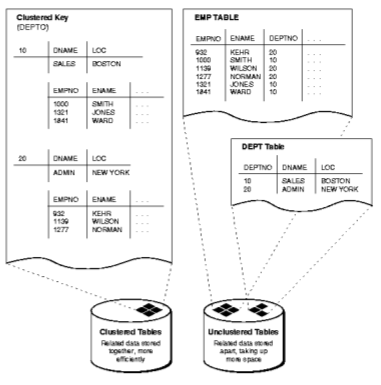
\includegraphics[scale=0.8]{images/2-cluster.PNG}
	\caption{Oracle: Clustered Tables.}
	\label{fig:cluster}
\end{figure}

\paragraph{Log Structured Databases}
Instead of storing tuples and modifying them as needed, only store a record of how the data is modified (a log). With this, inserts record the entire tuple, deletes indicate that a tuple is invalidated and updates record modified tuples (no in-place updates). New log entries are simply appended at the end of the log file (much faster than random access). Mainly used for in-memory OLTP (minimizes cost for making data persistent) and cloud storage (file storage is typically append only). Not useful for heavy OLAP. To optimize this concept, the log file is periodically compacted (remove history by adding only one entry for each tuple - all operations are applied) and the tuples and their modifications are indexed. %TODO more?

\paragraph{No Indexes}
Snowflake uses micro-partitions instead of indices (see previous section) and MonetDB (column store) uses database cracking: the index is built incrementally while the data is being processed on a column-wise basis. Initial queries are expensive but later cost us amortized as (some) work has already been done. See example in Figure \ref{fig:crack}. %TODO more?

\begin{figure}[h]
	\centering
	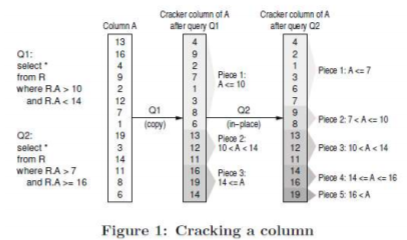
\includegraphics[scale=0.8]{images/2-crack.PNG}
	\caption{Database cracking example.}
	\label{fig:crack}
\end{figure}





\subsection{Reading Assignments}


\subsubsection{Modern B-Tree Techniques}


\paragraph{B-Tree vs. Hash Index}
Argument for hash index: single I/O per lookup and CPU efficient due to efficient comparisons and address calculations. But:
\begin{itemize}
    \item I/O: if branch nodes are in buffer, B-Tree is also single I/O.
    \item CPU: Just use hash values as keys (or other efficient keys).
    \item Straightforward space management.
    \item Multi-field indexes and nonuniform distributions of key values.
    \item Efficient index creation. Online creation possible.
    \item Support for ordered scans and range predicates.
    \item etc.
\end{itemize}

\paragraph{Key Normalization}
To reduce the cost of key comparisons, transform keys into binary strings s.t. simple binary comparisons suffice to sort the records during index creation and to guide a search. Key sequence for sort order of original key and binary string have to be the same and all comparisons equivalent. Binary strings may also encode multiple columns and additional information. Also allows for easy compression. %TODO example





\subsubsection{The Design and Implementation of Modern Column-Oriented Database Systems}

\paragraph{Compression Ratio}
CS has an improved compression ratio compared to RS since each column can be compressed in a different way. Since many compression ratios compress data in a non-fixed way, using virtual IDs to identify single items in a column becomes more complex.

\paragraph{Late Materialization}
Delay the joining of columns into wider tuples. Possible in CS since it allows for processing data in a columnar format.

\paragraph{C-Store}
\begin{itemize}
    \item Data on disk is represented as a set of column files with each file containing data from a single column - compressed in a column-specific manner and sorted on the column attribute. = Read Optimized Store (ROS)
    \item Newly loaded data is stored in Write Optimized Store (WOS) - uncompressed and not vertically partitioned.
    \item Both ROS and WOS are accessed when processing a query.
    \item Data is periodically moved from WOS to ROS by a tuple mover (sort, compress, divide and write to disk).
    \item A column may be stored several times in different sort orders (to process frequent queries efficiently).
    \item Projection = group of columns sorted on same attribute. There is at least one containing all columns and it can be used to answer any query.
    \item Column-specific compression depends on if column is sorted, its data type and the number of its distinct values.
    \item No secondary indexes on tables.
    \item Sparse indexes: indexing into sorted projections. It stores the first value contained on each physical page of a column.
    \item No-overwrite storage representation: updates are deletes followed by inserts. Deletes are processed by storing a delete column recording the time every tuple was deleted (if).
    \item Queries are run as of a specific time to filter out deleted tuples. This allows time travel.
    \item DB modification uses two-phase locking.
    \item Based on a shared-nothing architecture. Projections are horizontally partitioned.
\end{itemize}

\paragraph{MonetDB}
\begin{itemize}
    \item Data is stored column-wise both in memory and on disk (uncompressed on disk). Exploits bulk processing and late materialization. Profits from SIMD instructions. Push-based operators.
    \item No buffer pool, only memory-mapped files. %TODO Virtual mem?
    \item Column-at-a-time algebra.
    \item %TODO BAT Algebra stuff...
    \item Intermediate results are fully materialized. See materialized execution model.
    \item
    \item Processing algorithms, that minimize CPU cache misses rather than IOs
    \item Indexing, which is not a DBA task but happens as a by-product of query execution, i.e., database cracking
    \item Query optimization, which is done at run-time, during query incremental execution
    \item Transaction management, which is implemented using explicit additional tables and algebraic operations, so read-only workloads can omit these and avoid all transaction overhead
\end{itemize}

\paragraph{VectorWise}
\begin{itemize}
    \item Balance between full materialization of intermediate results as in MonetDB and the tuple-at-a-time iterator model. See vectorized execution model.
    \item Using Positional Delta Trees for updates.
    \item If there is an arithmetic operation only for small number of values selected in an array, VectorWise can compute this operation for all the array, even though it is not necessary.
    \item VectorWise tunes the vector size such that all vectors for evaluating a query together fit in the CPU cache.
    \item 
\end{itemize}

Loop pipelining → Mapping loops into optimized pipeline executions, Array blocking → Grouping subsets of an array to increase cache locality, Strength reduction → Replacing an operation with an equivalent less costly operation

The typical size of each vector in vectorized execution does not fit the L2 cache.

RLE: (value, start position, runLength) triples

Late materialization can benefit from selection and aggregation operators.


NSM: record header, DSM: record ID, columns, PAX: mini pages






\subsubsection{Data Page Layouts for Relational Databases on Deep Memory Hierarchies}


%TODO PAX wiki



\subsubsection{A Hybrid Page Layout Integrating PAX and NSM}

See Figure \ref{fig:pax} for difference between NSM and PAX.

\paragraph{PAX}
Each page is partitioned into n minipages (degree of relation). Values of the first attribute are stored in first minipage and so on. Page header contains pointers to beginning of each minipage. Fixed-length attributes are stored in F-minipages with a presence bit vector at the end for each entry - it indicates null values. Variable-length attributes are stored in V-minipages with pointers pointing to the end of each slot.

\paragraph{PAX Disadvantage}
Complexity of free space management withing a page for records with one or more variable-sized fields.

\paragraph{Hybrid Page Layout (HPL)}
Combines NSM and PAX. From NSM: two variable-sized allocation spaces growing towards each other. From PAX: cache efficiency during large scans.

\paragraph{Simple Segments}
Simplest HPL variant. Allocation space for fixed sized fields grows from one end, allocation space for variable sized fields from the other. Offsets for V-fields are their own fixed sized fields.


Set of records in the F fields is divided into segments. Number of records per segment = number of bytes per cache line. With 13 total bytes of F field values, we have 13 cache lines per segment.

%TODO






\subsection{Exercises}

\subsubsection{Column-Store}

\subsubsection{Page Layouts and Indexing}

\subsubsection{Indexing}

\newpage

\section{Query Processing}

We are now at the top two layers of Figure \ref{fig:arch}.


\subsection{Introduction}

To process / parse a query sent from a client (DB application), it is first allocated to a process / thread through a DB engine interface while validating it, checking access control (permissions) and matching it with the query cache. Then, for each uncached query, a query plan (operator tree) is created (possibly rewriting and optimizing the query) and executed while buffers are read from the DB buffer cache or from disk. Finally, the results are sent back to the client.

%TODO oracle / IBM example? images? make tree?

A DB engine is commonly a shared environment with many users running queries concurrently while the engine itself runs its own maintenance procedures. A DB engine is similar to an OS since it has to schedule, orchestrate and mediate access to shared resources.

In a commercial setting, DBs are used programmatically meaning that queries generated by user interfaces are created by application programs. The use of views and query templates affects query processing.


\paragraph{Caching}
In a DB system, it is very likely to receive the same query multiple times and sometimes even in a short time frame. The best way to speed up execution is to reuse results from a previous execution (parsing, optimization, query itself, (intermediate) results\footnote{Query results can be cached in the engine itself or outside of it (intermediate layer, client-side caching, etc.).}, etc.) - everything can be cached! This also works well for data that does not change much (e.g. BLOBS / large data items). As always, consistency problems have to be dealt with.

%TODO oracle / amazon / microsoft example for outside engine caching? more on client caching

\paragraph{Processes vs. Threads}
\begin{itemize}
    \item \textbf{OS Process:} A program execution unit scheduled and managed by the OS with a private and unique address space and its own state.
    \item \textbf{OS Thread:} A program execution unit part of a multi-threaded process that shares its address space and context with other threads from the same process. Scheduled and managed by the kernel.\footnote{Kernel: core program of an OS with complete control over everything in the system. It connects the application software to the hardware (CPU, memory, devices).}
    \item \textbf{Client Process:} Execution unit running on client / application side used to connect to the DB engine.
    \item \textbf{Server Process:} Execution unit running inside the DB engine, used to execute queries on behalf of a client. A query can be processed by several server processes (parallel execution) a.k.a. a pool.
    \item Potentially confusing: the two things above can also be threads in a DB context!
\end{itemize}

With concurrent users, a DB system can be designed to either use a process or a thread for each user session. When using processes, we can take advantage of their isolation and security properties but scalability is limited, context switching is slow (lots of state is maintained) and implementation of parallel query processing is more complex. Furthermore, in a DB context, many data structures are shared across processes (buffer cache, lock table, common memory pools, etc.), which goes against the notion of processes. Most modern systems use threads (shared state and memory facilitates access to common data structures and parallel query processing, lightweight, scalability, etc.) - but more complex management in terms of isolation.

%TODO oracle, postgres example? session definition?

\paragraph{Memory Structures}
Memory needs to be managed carefully since we have many different things running at the same time and shared vs. local memory has to be differentiated. It is common to divide it into regions each with a single purpose.

%TODO oracle example pga (cursor), sga, DB instance, etc.

\paragraph{Cursor}
A pointer to a data structure (table, view, result, etc.) used to navigate the structure - similar to the iterator concept in programming languages. Space needs to be allocated to manage its state (opened, closed, accessed, etc.). When a table is processed, a cursor moves from tuple to tuple. Also used when delivering results to clients - instead of returning a possibly huge table, the cursor to it is returned. %TODO more?


\subsection{Execution Models}

When processing an SQL query, it is parsed into a tree of operators which is the basis for the execution model (see Figure \ref{fig:tree}). The leaves are the tables involved in the query and the root is the final result. Typically, each operator has at most two input from the lower layers (join). Operators can read input / output results one tuple at a time or as a whole - some are even blocking (all operations need to be completed until result can be issued). Each query and each subtree is its own table.

\begin{figure}[h]
	\centering
	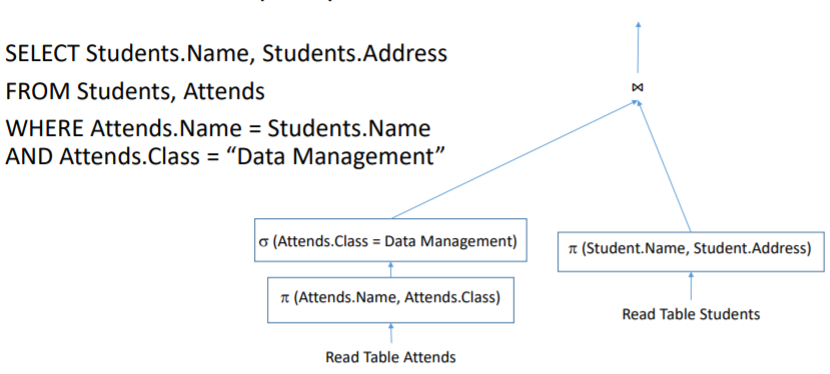
\includegraphics[scale=0.6]{images/3-tree.PNG}
	\caption{Query plan of an example SQL query.}
	\label{fig:tree}
\end{figure}

\paragraph{Pull Mode}
An operator obtains data through a function call to a lower operator (control moves top-down) - data is obtained whenever it is needed. Good for disk-based systems and whenever the data doesn't fit in memory.

\paragraph{Push Mode}
A lower operator sends its result up as soon as it completes processing a tuple / buffer / vector. Higher operators receive results and potentially have to buffer them if they're not ready yet to process them. Can be more efficient than pull mode (hardware / CPU exploitation) but it's more difficult to implement (buffer, synchronization, etc.) - similar to event-based programming. %TODO hardware exploitation


\subsubsection{Single Machine Execution Models}

%TODO operator implementation? if not later

\paragraph{Iterator Model (or Volcano / Pipeline)}
Tuples = data traverse the tree from leaves to the root. Operators iterate over those tuples to process them by using the interface \texttt{Next()}. The execution (control) is top-down (the \texttt{Next()} call initiated at the top trickles down until it can be executed). Once both tables (left and then right) are filled, the nested for-loop is executed. Widely used in disk-based systems and works for all workloads. See Figure \ref{fig:iterator}.

\textbf{Pros:} Generic interface for all operators (great information hiding). Iterators are easy to implement. Supports buffer management strategies. No overhead in terms of main memory. Supports pipelining, parallelism and distribution (with special iterators).

\textbf{Cons:} High overhead of method calls (context switches) and poor instruction cache locality (jumping down and up in the tree calling different functions).

\begin{figure}[h]
	\centering
	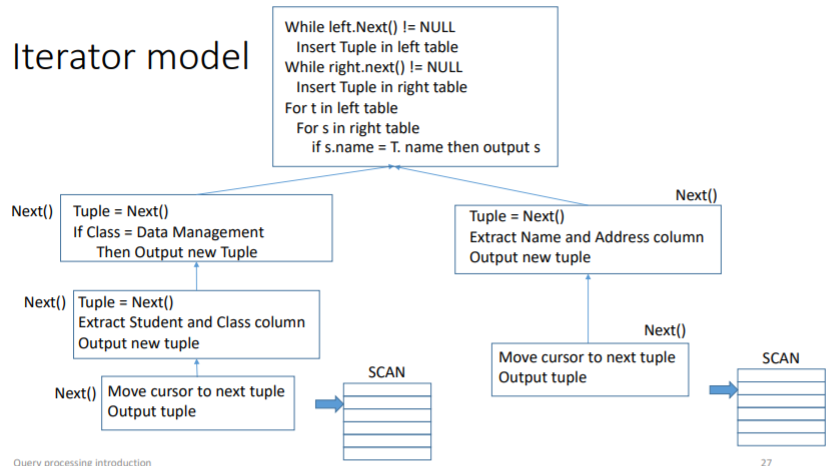
\includegraphics[scale=0.7]{images/3-iterator.PNG}
	\caption{Iterator model of example SQL query (typo: "Name" instead of "Student" in left block).}
	\label{fig:iterator}
\end{figure}

\paragraph{Materialization Model}
Similar to the iterator model but instead of outputting one tuple at a time, each operator outputs its result in a single buffer (each operator is called only once). Much less method calls - less overhead than previous model. Works well in OLTP (queries / transactions process small amounts of data resulting in small buffers that are passed around) - assuming data fits in memory. Not suitable for OLAP since data being passed around can be very large. See Figure \ref{fig:material}.

\begin{figure}[h]
	\centering
	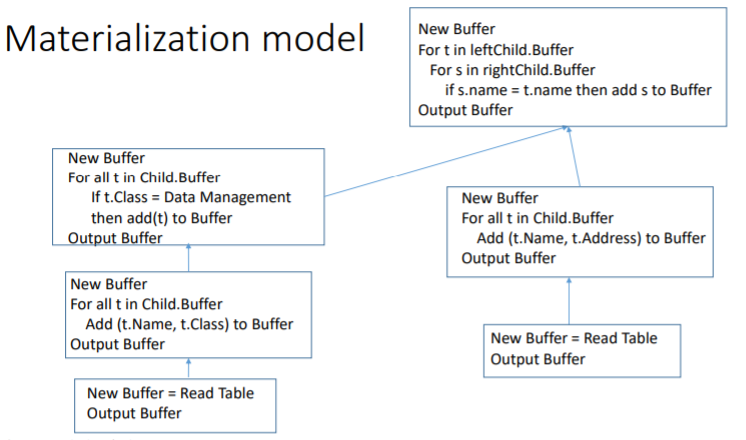
\includegraphics[scale=0.7]{images/3-material.PNG}
	\caption{Materialization model of example SQL query.}
	\label{fig:material}
\end{figure}

\paragraph{Vectorized / Batch Model}
Exploits SIMD / AVX (and column-store) by combining the iterator and materialization model. Data is iterated over with \texttt{Next()} which returns a set of tuples (e.g. entire column) instead of a single one resp. a full buffer. This works best for OLAP systems. %TODO example?


\subsubsection{Parallel Processing Execution Models}

To parallelize a plan or distribute it across several machines, the above models can simply be extended with an \texttt{EXCHANGE} operator. The operator only moves data from one place (e.g. machine) to another - it does not modify data. See Figure \ref{fig:exchange}.

\begin{figure}[h]
	\centering
	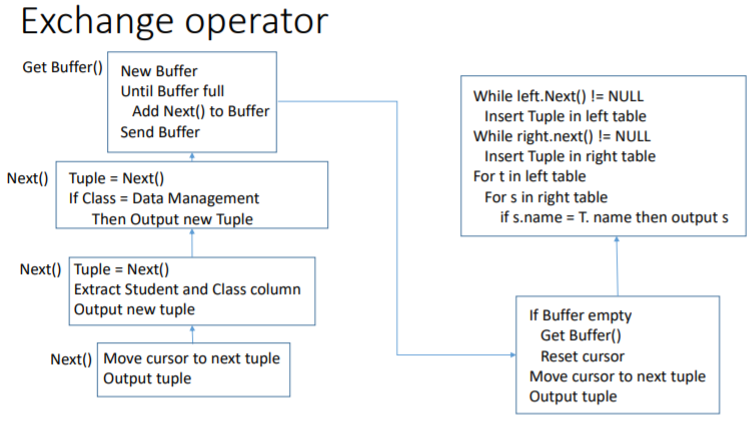
\includegraphics[scale=0.7]{images/3-exchange.PNG}
	\caption{One way to implement an exchange operator (as a driver) shown with example SQL query.}
	\label{fig:exchange}
\end{figure}


\subsection{Query Optimization}

Since SQL is declarative, a DB engine has many options to translate a query into an executable program. After generating possible execution plans for a query, the best one has to be chosen (based on rules or based on estimated cost). A plan is influenced by the access methods for each table (leaves of the query tree), i.e. available indices, predicates, clustered tables (same extent), type of operator implementation, i.e. join implementation, sorted data, and the shape and form of the query tree.

\paragraph{View}
The result set of a stored query on the data (virtual table). A view can be queried just like any other persistent database collection object. Changes applied to the relevant underlying data are perpetuated. A view can me materialized into an actual table and added to the schema (usually done for common operations over the schema). Mainly used to implement logical data independence (create schema different from original one) and access control (access view instead of base tables). %TODO more on why? SQL command

\paragraph{Schema}
A schema is made up of base tables defined at the beginning. It provides the basic organization of the data. Views allow to tailor that logical organization to the needs of particular applications without changing the basic schema. The more complicated a schema is, the more extensive is the use of views. 

%TODO examples: TPC-H, TPC-C/star, snowflake, TPC-DC/snow storm, dimension and fact tables


\subsubsection{Query Rewriting}

After a query has been parsed, it is often rewritten into an equivalent query based on the DB schema and on some heuristics. The rewritten query is then used as input for the query optimization process. 

Rewriting can remove operations to make the query more efficient, can give the optimizer more freedom to operate, can make the query's intent more explicit and can map it to actual base tables and views as needed / for efficiency reasons.

\paragraph{Rewriting Predicates}
A predicate has to be checked for every tuple. The query will run faster if we either reduce the number of comparisons that need to be made and / or if we avoid going several times over the same tuple to check a different predicate. Predicates can be fully transformed or augmented (transitive closure) to decrease the number of comparisons. Augmentation gives the optimizer more options to consider (A=B, B=C - also add A=C; A=B, B$>$100 - also add A$>$100; etc.). Examples in Figures \ref{fig:transormation}, \ref{fig:aug1} and \ref{fig:aug2}.

\begin{figure}[h]
	\centering
	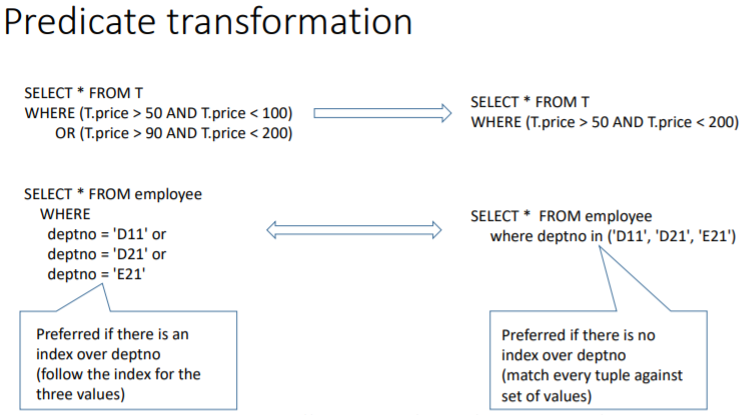
\includegraphics[scale=0.5]{images/3-transformation.PNG}
	\caption{Predicate transformation example.}
	\label{fig:transormation}
\end{figure}

\begin{figure}[h]
	\centering
	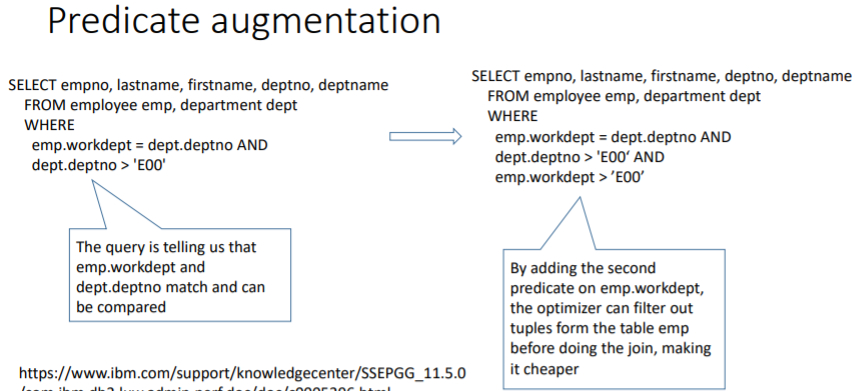
\includegraphics[scale=0.5]{images/3-aug1.PNG}
	\caption{Predicate augmentation example 1.}
	\label{fig:aug1}
\end{figure}

\begin{figure}[h]
	\centering
	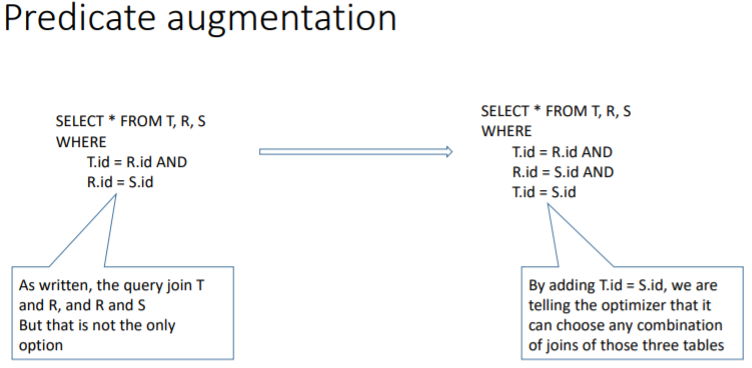
\includegraphics[scale=0.5]{images/3-aug2.PNG}
	\caption{Predicate augmentation example 2.}
	\label{fig:aug2}
\end{figure}

%TODO more examples from slides

\begin{itemize}
    \item Predicate transformation
    \item Predicate augmentation
    \item Arithmetic changes (sum, count, avg)
    \item Predicate pushdown / view folding (view to base table for single pass)
    \item Query unnesting
    \item Materialized views rather than base table %TODO example
    \item Remove distinct if attribute is key
    \item etc. %TODO more "tips"
\end{itemize}


\subsubsection{Rule Based Optimization: Heuristics}

With relational algebra, we can prove equivalence over queries (equivalence rules). This enables query transformations with the guarantee that the results stay the same.

%TODO cheat sheet? examples

\begin{itemize}
    \item Conjunctive selection operations can be deconstructed into a sequence of individual selections.
    \item Selection operations are commutative thus can be applied in a different order.
    \item Selection of a cartesian product = theta join.
    \item Selection of a theta join = theta join with both predicates in conjunction.
    \item Theta / natural joins are commutative.
    \item Natural joins are associative.
    \item Theta joins are associative in a special manner: %TODO
    \item %TODO etcetc
\end{itemize}


\subsubsection{Cost Based Optimization}

To choose the best query plan out of multiple equivalent ones for a query, we might rely on its estimated cost based on many types of information.

\paragraph{Statistics}
Statistics that are constantly collected on tables, indices, buffers and the system itself can be an information source for query optimization (which plan and which operator implementation). We have:

\begin{itemize}
    \item \textbf{Table Statistics:} Number of rows / blocks / etc., average row length, etc.
    \item \textbf{Column Statistics:} Number of distinct values / nulls / etc. (helps to estimate selectivity of a predicate or to decide on join order), data distribution (histogram), etc.
    \item \textbf{Extended Statistics:} Index statistics, number of leaf blocks, levels, clustering factor, etc.
    \item \textbf{System Statistics:} I/O performance and utilization, CPU performance and utilization, etc.
\end{itemize}


\paragraph{Histogram}
Help in cardinality estimation (CE), especially with skewed data. By default, uniform distribution of rows across the distinct values in a column is assumed

%TODO






\subsubsection{Operators}




%TODO





\subsection{Reading Assignments}

\subsubsection{Sort vs. Hash Revisited}

\subsubsection{Query Optimization}

\subsubsection{The State of the Art in Distributed Query Processing}

\subsection{Exercises}

\subsubsection{Query Processing}

\subsubsection{Query Rewriting}

\subsubsection{Query Optimization}

\subsubsection{Cost-Based Optimizer}

\subsubsection{Query Operators}
\newpage

\section{Transaction Management}

\subsection{Introduction}

In the previous section, we focused on queries used to access the DB with the purpose of reading data (optimization, data movement, indices). In this section, we focus on transactions. Transactions are accesses to the DB with the purpose of modifying the data (update, insert, delete). Important is: correctness, recovery and state management.

Concurrency control and recovery are deeply interrelated. CC implementation affects recovery implementation and recovery implementation restricts what can be done in terms of CC.

\begin{figure}[h]
	\centering
	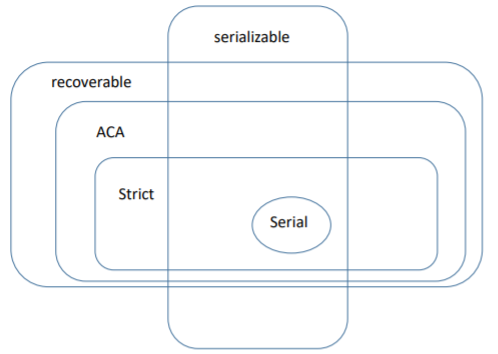
\includegraphics[scale=0.6]{images/4-histories.PNG}
	\caption{Consistency and recoverability properties.}
	\label{fig:histories}
\end{figure}




\subsection{Transaction Model}

\paragraph{Transaction}
A unit of work made up of multiple operations (read and / or write) that has all the properties specified by ACID - operations inside the same transaction cannot be reordered. A transaction can either commit, i.e. its changes are made persistent, or abort / rollback, i.e. it is cancelled and all changes are reverted. Some systems include the concept of a savepoint, i.e. temporarily committing changes until a certain point with the possibility of rollback to a savepoint.

\paragraph{Transaction Manager}
Enforces concurrency control in a DB engine. It includes (see Figure \ref{fig:manager}):
\begin{itemize}
    \item \textbf{Transaction Table:} List (commonly in common area) of active transactions in the system.
    \item \textbf{Transaction Handler:} Pointer to the structures containing all the relevant info related to a transaction (possibly in private area).
    \item \textbf{Lock Table:} Hash table containing entries that correspond to active locks. Locks on the same item = linked list.
    \item \textbf{Log:} Entries that capture the operations performed and are kept in memory until they're written back to disk.
\end{itemize}
A transaction manager goes through the following operations:
\begin{itemize}
    \item \textbf{Begin T:} Create entry in transaction table (no log entry unless explicitly requested).
    \item \textbf{Read/Write:} Hash tuple ID to find corresponding entry in lock table. If empty: grant lock to T, else: attach request to list and grant request if compatible.
    \item \textbf{Write:} Create log entry (with LSN, before/after image, transaction ID, pointers to previous log entry of same T, etc.).
    \item \textbf{Commit T:} Release lock, potentially resume transactions waiting for lock, finalize log entries, write log entries to storage, potentially write modified data to storage, etc.
    \item \textbf{Abort T:} Release lock, potentially resume transactions waiting for lock, use log entries to undo/discard changes, potentially write log entries to storage, etc.
\end{itemize}

\begin{figure}[h]
	\centering
	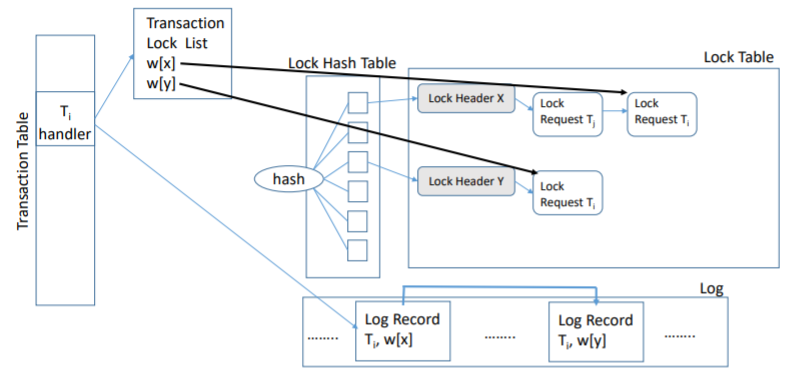
\includegraphics[scale=0.7]{images/4-manager.PNG}
	\caption{Basic functions of a transaction manager.}
	\label{fig:manager}
\end{figure}

%TODO more on lock table? other trans. manager designs

\paragraph{Conflicts}
\begin{itemize}
    \item \textbf{Write-Read (WR) / Dirty Read:} T2 reads object modified by T1 before T1 committed.
    \item \textbf{Read-Write (RW) / Unrepeatable Read:} T1 reads object that is modified and committed by T2, T1 then reads the same object again which results in a different value.
    \item \textbf{Write-Write (WW) / Lost Update:} T1 modifies an object previously modified by T2 with T1 committing before T2.
\end{itemize} 
If no write is involved, read-read (RR) does not cause a conflict.

%TODO abort / commit conflicts

\paragraph{History / Schedule} %SUMMARY image, serial vs. recover
A partially ordered sequence of operations from a set of transactions. 



\subsection{Concurrency Control}

How to ensure that the data remains consistent (data integrity) with a number of transactions and queries running at the same time.

\paragraph{ACID}
A set of properties of transactions intended to guarantee data validity despite errors, power failures and other mishaps. See Figure \ref{fig:acid}.

\textbf{Atomicity:} (Group of) operations taking place in their entirety or not at all. Intermediate states are not guaranteed to be correct. Atomicity requires isolation meaning that intermediate state should never be seen by another transaction.

\textbf{Consistency:} Assumption that an accepted transaction is correct (according to all defined rules / constraints).

\textbf{Isolation:} Property defining how / when the changes made by one operation become visible to others. Usually, transactions will be executed as if they were alone (intermediate state is not visible). Isolation is enforced with locking mechanisms.

\textbf{Durability:} Guarantee that transactions that have committed will survive permanently. Usually handled with some kind of logging mechanism, i.e. capturing consistent states in snapshots.

\paragraph{Serial History}
A history is serial if for every two transactions that appear in it either all operations of the first one appear before all operations of the second one or vice versa. By definition, a serial history with only committed transactions is correct (isolation, transactions start and end in a consistent state).

\paragraph{Equivalent Histories}
Two histories are equivalent iff they include the same transactions containing the same operations and conflicting operations of non-aborted transactions are ordered the same way in both histories. This implies that committed transactions in either history see the same state and leave the DB in the same state (same effects).

\paragraph{Conflict Equivalent Histories}
One can be transformed to the other by swapping non-conflicting operations.

\paragraph{Serializable History}
History is serializable iff it is equivalent to a serial history. If it is, it is correct (leaves the DB in a consistent state). %TODO commit included?

\paragraph{Serializability Graph}
A compact representation of the dependencies in a history. One node per committed transaction. Edge from T to T' if an action of T precedes and is in conflict with an action of T'. %TODO examples

\paragraph{Serializability Theorem}
A history is serializable iff its serializability graph is acyclic. Sorting it topologically results in an equivalent serial history.

\paragraph{Conflict Serializability}
If a history can be transformed into a serial history by swapping non-conflicting operations it is conflict serializable.



\subsection{Recovery}

How to ensure that the data remains consistent even when unexpected failures occur. A.k.a. changes from transactions that have not completed are not visible and changes from committed transactions are recorded and visible.

\paragraph{Types of Failures}
\begin{itemize}
    \item Transaction failure (abort, fail, time out, etc.) - undo its changes.
    \item System failure - bring DB back to a consistent state (undo and redo).
    \item Media failure (disk fail, permanent storage has errors, etc.) - restore DB to a known consistent state (replication, separating data from log files, etc.).
\end{itemize}

\paragraph{Recovery Procedures}
\begin{itemize}
    \item \textbf{R1:} Undo all changes from a single transaction - regardless of why.
    \item \textbf{R2:} Redo changes from committed transactions in case of a system crash where main memory is lost and disk is kept.
    \item \textbf{R3:} Undo the changes that remain in the system from active transactions in case of a system crash where main memory is lost and disk is kept.
    \item \textbf{R4:} Read consistent snapshots from backup and if possible apply the log (in case of system crash with loss of disk).
\end{itemize}

\paragraph{Undo vs. Redo}
To ensure atomicity in case of a non-completed transaction, we either need to: restore the initial DB state and remove any effects of the transaction (before image) or reach the intended final state of the transaction in question. Redo might also be applied to restore the changes of already committed transactions (after image).

\paragraph{Recoverable History (RC)}
If T2 reads an object modified by T1 and commits, T1 committed before T2 did. A committed transaction does not need to be undone since it cannot read wrong data and transactions commit in their serialization order.

\paragraph{Avoids Cascading Abort History (ACA)}
If T2 reads an object modified by T1, the read has happened after T2 committed. Aborting a transaction does not cause aborting others and transactions only read from committed transactions.

\paragraph{Strict History (ST)}
If T2 reads / writes an object modified by T1, the operation has happened after T2 committed or aborted. Undoing a transaction does not undo the changes of other transactions and transactions do not read / write updates of uncommitted transactions.

\paragraph{SQL Isolation Levels (ANSI)}
%TODO

\paragraph{Logging}
In case of system failure (sudden loss of data in memory) the engine needs to recover the DB up to the point of its last committed state which includes all changes made by all committed transactions up until time of failure = recovery procedure. The recovery procedure can only operate with data on permanent storage and needs to be correct even if successive failures occur in the middle of it. To do this, we need to be able to do logging.

%TODO serial. strict p6? when to write undo redo shit

\paragraph{Recovery Procedure}
A recovery procedure implemented by a recovery manager requires either undo and redo, just undo or just redo or neither. Undo needs before images (write back before commit) and redo needs after images (write back after commit). %TODO steal and force

\paragraph{Undo and Redo}
\begin{itemize}
    \item \textbf{Read:} Simply read value from block on buffer cache.
    \item \textbf{Write:} Create log entry (before and after image) and append to persistent log. Write after image to block on buffer cache.
    \item \textbf{Commit:} Write persistent log entry indicating that T has committed.
    \item \textbf{Abort:} For all updates, restore the before image using the log entry.
\end{itemize}
The recovery procedure will start from the end of the log and work backwards and keep two lists: undone items and redone items. Procedure terminates when all items are in either list or we're at the beginning of the log. For each log entry: if the accessed item is not yet in a list apply after image and add to redone list if it is part of a committed T or apply before image and add to undone list if it is part of an aborted T. %TODO pros

\paragraph{Just Undo}
\begin{itemize}
    \item \textbf{Read:} Simply read value from block on buffer cache.
    \item \textbf{Write:} Create log entry (before image) and append to persistent log. Write after image to block on buffer cache.
    \item \textbf{Commit:} Flush all dirty values modified by T if still in cache. Write persistent log entry indicating that T has committed.
    \item \textbf{Abort:} For all updates, restore the before image using the log entry.
\end{itemize}
Procedure same as above just with one undone list - each item part of an aborted T is restored to before image and added to this list. This relies on the fact that all committed values are in persistent storage and have not been lost. Works if strict execution is assumed. %TODO comments

\paragraph{Just Redo}
\begin{itemize}
    \item \textbf{Read:} If T has not written value before, read it from buffer cache. Else: read value from temporary buffer.
    \item \textbf{Write:} Create log entry (after image) and append to persistent log. Write after image to some temporary buffer.
    \item \textbf{Commit:} Apply all updates in temporary buffer to actual data blocks. Write persistent log entry indicating that T has committed.
    \item \textbf{Abort:} Discard temporary buffer.
\end{itemize}
Procedure same as above just with one redone list - each item not in list and part of a committed T is added to list and changes are redone using before image. Relies on never having dirty blocks in buffer cache - all data there is committed and is the most recent version. %TODO comments

\paragraph{Neither}
Rare resp. not used in practice, does not require a log and also there is no recovery procedure (that's the point). Uncommitted data is never written to persistent storage and data in memory is never dirty. Requires ability to write all changes made by a transaction to persistent storage in a single atomic action. %TODO data structures
\begin{itemize}
    \item \textbf{Read:} If T has not written value before, use current directory to find latest committed copy. Else: use shadow directory of T to find updated copy.
    \item \textbf{Write:} Write to buffer and add pointer to shadow directory of T.
    \item \textbf{Commit:} Create full directory by merging current one and shadow one of T. Swap pointer indicating latest committed directory.
    \item \textbf{Abort:} Discard buffer and shadow directory.
\end{itemize} %TODO comments

\paragraph{Log Record}
Log sequence number (LSN) for navigation, system change number (SCN) for event timestamps (T start), pointers to other log records of same T, transaction ID and related info (redo: change vectors = after images - describes changes to single block of data, undo: before images).
%TODO log blocks. more on SCN

\textbf{In Memory:} %TODO
\textbf{In Storage:} %TODO

%TODO




\subsection{Locking}

Concurrency control in DBs is implemented using locking (usually with a lock table as seen in a transaction manager).

\paragraph{Compatibility Matrix}
%TODO lock modes? granularity stuff

\paragraph{Two Phase Locking (2PL)}

\paragraph{Strict 2PL}

\paragraph{Deadlock Detection}

\paragraph{Snapshot Isolation}







\subsection{Reading Assignments}

\subsubsection{Concurrency Control and Recovery in Database Systems}

\subsection{Exercises}

\subsubsection{Serializability and 2PL}

\subsubsection{Recovery}
\newpage


\end{document}

